\section{Introduction}
\label{sec:intro}

American Sign Language (ASL) is the predominant language of Deaf communities in the United States, with an estimated 500,000 native users~\cite{ethnologue}. However, natural language processing has largely focused on spoken and written language only~\cite{yin2021including}. Recently, there is an increasing body of work in NLP tasks related to sign language, with particular focus on isolated sign language recognition (ISLR) and sign language translation (SLT).

In ISLR, the input consists of dictionary-style videos which have only one signer articulating one individual sign, and the task is to classify this video according to the sign label. Figure~\ref{fig:wlasl-samples} shows frames extracted from such videos, which are typically two or three seconds long, have a solid color background, and show people signing while standing facing the camera. ISLR labels are usually words in English or sign language glosses, which are typically a combination of morpheme translations into English along with differentiating phonological features like handshape and location.

\begin{figure}
    \centering
    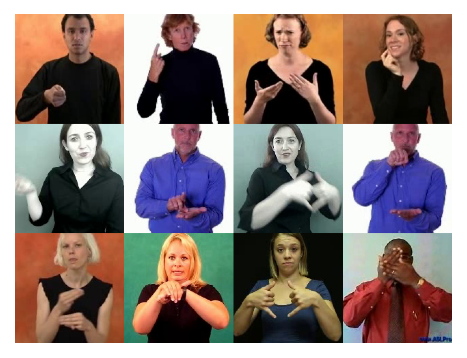
\includegraphics[width=\linewidth]{figures/wlasl-samples.pdf}
    \caption{Sample frames from isolated sign language video extracted from the WLASL2000 dataset~\cite{Li2020WLASL}.}
    \label{fig:wlasl-samples}
\end{figure}

On the other hand, in SLT the input consists of videos that contain continuous signing, and the task is to produce (usually text) translations in a given target language, typically the lingua franca of the region where the source sign language is predominant or English. The sources of these videos are highly variable, ranging from news sources to personal video blogs. Figure~\ref{fig:oasl-samples} shows example frames from sign language translation videos. Unlike ISLR, these videos are significantly longer, and can include all sorts of backgrounds, positions, and number of people, depending on the source it was extracted from.

\begin{figure}
    \centering
    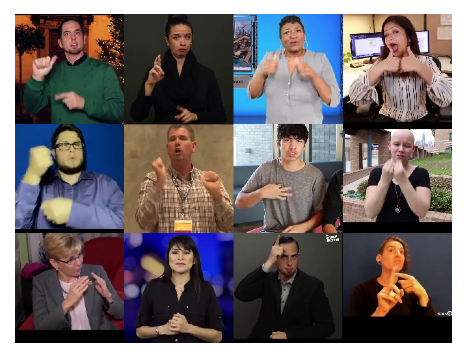
\includegraphics[width=\linewidth]{figures/oasl-samples.pdf}
    \caption{Sample frames extracted from ASL to English translation dataset OpenASL~\cite{Shi2022OpenASL}.}
    \label{fig:oasl-samples}
\end{figure}

In this paper, we focus on ISLR as a task to evaluate our models, as translation remains extremely difficult, with very poor state-of-the-art performance. Moreover, SLT models often rely on ISLR models as feature extractors~\cite{chen2022simple,muller2022findings,shi2022ttic}. Despite their usage in a language task, these models have not yet been evaluated in their ability to encode linguistically relevant features. In the case of sign languages, Brentari's prosodic model of sign language phonology~\cite{brentari1998prosodic} provides a set of phonological features that can uniquely characterize up to 70\% of signs in ASL~\cite{sehyr2021asllex}. These encode multiple characteristics of all signs, such as handshapes, movement, and symmetry.

Naturally, the most common modality of sign language data is video. Current state-of-the-art video classification tasks are dominated by vision transformers. Recent advances in this area have come from various self-supervised pre-training tasks, especially when dealing with smaller classification datasets. These are either based on some form of contrastive pre-training~\cite{pan2021videomoco,Kuang_2021_ICCV,Ranasinghe2021SVT} or masked reconstruction~\cite{Tong2022VideoMAE,Wang2021BEVT,Wei2022MaskFeat}, following the nature of advances in other fields like text, single images, and speech. These self-supervision methods have not yet been explored for sign language tasks. Self-supervision requires large datasets to function effectively, and large sign language datasets did not exist until very recently. In this paper, we study multiple video transformers and self-supervision settings to understand the effect of self-supervision for sign language processing tasks.

The contributions of this paper are the following:
\begin{itemize}
    \item \textbf{Establish a new state of the art on gloss-based WLASL2000.} MViTv2 with MaskFeat pre-training achieves 79.02\% accuracy, surpassing pose-based state of the art by 1.59\%.
    \item \textbf{Evaluate the effect of multiple self-supervision tasks on ISLR performance.} We compare pixel reconstruction (VideoMAE~\cite{Tong2022VideoMAE}), feature reconstruction (MaskFeat~\cite{Wei2022MaskFeat}), BERT pre-training for videos (BEVT~\cite{Wang2021BEVT}), and DINO pre-training for videos (SVT~\cite{Ranasinghe2021SVT}).
    \item \textbf{Introduce phonological features as a tool to analyze sign language representations produced by self-supervised models.} We use this to better characterize the strengths and limitations of architectures and pre-training tasks.
\end{itemize}
